\documentclass{article}
\usepackage{geometry}
\usepackage{fancyhdr}
\usepackage{amsmath, amsthm, amssymb}
\usepackage{graphicx}
\usepackage{hyperref}
\usepackage{courier}
\usepackage{color}

\title{MLEND Capstone Project: Training a Smartcab Planner}
\author{Lucas Murtinho \\ \url{lucas.murtinho@gmail.com}}
\date{\today}
\begin{document}
\maketitle
\tableofcontents
\newpage

\section{Definition}


\subsection{Project Overview}

In Project 4 of Udacity's Machine Learning Engineer Nanodegree, I had to teach a smartcab in grid-like world how to get to a destination on time by obeying traffic rules and following the directions passed by a planner. Without any kind of hard programming, the agent should learn right-of-way rules and to go straight when the planner sent a "forward" input, for instance.

A natural extension of this project is, instead of relying on an outside planner, coming up with an agent that, given the smartcab's location and destination, learns how to plan a route. This is the goal of my capstone project.


\subsection{Problem Statement}

The problem at hand is to program an agent that learns to identify what the next waypoint should be for a smartcab in a grid-like world to reach its destination as fast as possible. I'll use an $8\times6$ grid for the project, similar to the one used for the Nanodegree Project 4, but in principle the solution should apply to a grid of any size.


\subsection{Metrics}
\label{sec:metrics}

I used the following metrics to gauge the performance of the learning planner:

\begin{itemize}
    \item The number of \textbf{destinations reached} over all trials.
    \item The \textbf{number of steps needed} to reach the destination.
    \item The \textbf{sum of rewards}  over each trial.
    \item The number of trials with \textbf{net positive rewards}.
    \item The number of \textbf{states visited} by the planner.

\end{itemize}

I computed these metrics over 1000 trials, setting the deadline to 100 steps for each trial. In an $8\times6$ grid, this number of steps is largely sufficient for any reasonable planner to have the agent reach its destination.

It's worth noting that some of these metrics are a means to an end. Ultimately, a successful planner is one that leads the agent to its destination in the shortest number of steps. Therefore, we can consider the number of destinations reached and the time left when the agent reached its destination as \textit{first-order metrics}, which are directly measuring what we want the planner to achieve.

On the other hand, metrics pertaining to the sum of rewards received by the planner during the trials are \textit{second-order metrics}, since the rewards' only purpose is to push the agent towards the desired behavior. Such metrics may indicate a problem in our algorithm: if the rewards are largely positive but the agent fails to reach its destination, or does so through a non-optimal path, we may have to change how rewards are defined.

The number oF states visited falls somewhere between these two categories of metrics. One could argue that a successful planner is also one with an extensive knowledge of the state space, since otherwise the agent can be ``caught by surprise'' in later trials, when it reaches a previously unknown state. 

\section{Analysis}

\subsection{Input Space Description}

In Project 4 of Udacity's Machine Learning nanodegree, the world in which the smartcab existed was represented by a graphical $8\times6$ grid rendered in Pygame. I'll use an image of that world in the \hyperref[sec:explovis]{next section}, but for now I'll describe the problem's input space abstractly.

\subsubsection{Position and Heading}

In the grid-like world of the smartcab, each position is defined by an $(i, j)$ tuple, in which $i$ is the longitude (the position across the East-West axis) and $j$ is the latitude (the position across the North-South axis). In a $m\times n$ grid, $(1, 1)$ represents the northwesternmost position, while $(m, n)$ represents the southeasternmost position.

The goal, then, is that, given a position tuple $(i_{cab}, j_{cab})$, a destination tuple $(i_{dest}, j_{dest})$, and a heading (described below), the planner should be able to come up with the best next action for the smartcab: \texttt{forward}, \texttt{right}, or \texttt{left}. 

The results of an action taken by the smartcab depends on its heading. The heading is a tuple $(i_{head}, j_{head})$, whose items represent East-West heading and North-South heading, respectively. The heading tuple must obey the following rules to be valid:

\begin{enumerate}
   \item The value of a tuple element indicates how the smartcab will move along the element's axis if it moves forward. This value can be either -1, 1, or 0.
   \item If the first element of the tuple is non-zero, the second element is zero and vice-versa. (This means the smartcab can only be headed in one direction at a time.)
\end{enumerate}

These rules imply four valid headings: $\{(1, 0), (-1, 0), (0, 1), (0, -1)\}$. These headings indicate the smartcab is turned East, West, South, and North, respectively.
 
Therefore, if the smartcab is at position $(i_{cab}, j_{cab})$ and moves forward, at the next step it will be at position $(i_{cab} + i_{head}, j_{cab} + j_{head})$ - with an important exception: the grid world is \textit{toroidal}, which means going "over the border" will bring the smartcab to the other side. If the smartcab is headed East at the eastnorthernmost position $(8, 1)$ in an $8\times6$ grid, for instance, moving forward will bring it to the westnorthernmost position $(1, 1)$. 

The more general formula for the smartcab's position at the next step after moving forward (considering, as stated above, that $(1, 1)$ represents the northwesternmost position in an $m\times n$ grid) is therefore:

\begin{equation}
((i_{cab} + i_{head} - 1) \% m + 1, (j_{cab} + j_{head} - 1) \% n + 1)
\end{equation}

The above expression is used to update the smartcab's location in the current version of the environment class used for project 4 (see \href{https://github.com/udacity/machine-learning/blob/2b6a7fca8ea43e00519f426a6b4ad3a130fca737/projects/smartcab/smartcab/environment.py#L195-L19}{here}).

\subsubsection{The \texttt{PlannerWorld} Class}

To define the input space in which the planner is to operate, I created the \texttt{PlannerWorld} class, with the following attributes and methods:

\begin{itemize}
    \item \texttt{grid\_size}: a tuple defining the size of the grid (East-West and North-South).
    \item \texttt{trials}: the number of trials to run.
    \item \texttt{deadline}: the number of steps an agent is allowed to take in each trial. If the agent takes \texttt{deadline} steps without reaching its destination, the trial is terminated.
    
    \item \texttt{get\_delta()}: given the agent's location and its destination, this method returns a tuple with the shortest East-West and North-South distances between these two points. If the shortest distance is going East or South, the corresponding element in the returned tuple is positive; if the shortest distance is going West or North, the element is negative. (In other words, delta has the same sign as the heading the agent should be in order to take the shortest path to its destination.)
    
    \item \texttt{get\_distance()}: given a delta tuple, this method returns the Manhattan distance between the agent's location and its destination. It will be used to compute the reward the agent will receive at each step of a trial.
    
    \item \texttt{get\_reward()}: this method returns a reward according to the state the agent is in. If the agent has reached its destination, the reward is the number of steps the agent still could take before the termination of the trial (or \texttt{deadline}  minus the number of steps taken in the trial). If the agent has not reached its destination, the reward is the negative of the Manhattan distance between the agent's location and its destination. 
    
    \item \texttt{move\_agent()}: this method will update the agent's position and heading according to the action taken by the agent and to the agent's heading when said action was performed. For instance, if the agent is at position $(1, 1)$, facing North, and goes right, its next position will be $(2, 1)$ and its next heading will be to the East. The method takes into account the toroidal nature of the world and allows the agent to "go across" the world's boundaries.
    
    \item \texttt{get\_random\_position()}: this method returns a random position in the world. For an $m\times n$ world, the northeasternmost position will be $(1, 1)$ and the southwesternmost position will be $(m, n)$.

    \item \texttt{simulate()}: this method simulates the agent's world. For as many trials as defined in the world's \texttt{trial} attribute, the method performs the following:
    
    \begin{itemize}
        \item The agent's location and its destination are randomly initialized using \texttt{get\-\_random\-\_position()}, and the agent's heading is also randomly defined
        \item The sum of rewards for the trial is defined as 0
        \item For each step in the trial:
        
        \begin{itemize}
            \item The delta tuple is calculated using \texttt{get\_delta()}
            \item The state is defined as a tuple containing the delta tuple and the agent's heading
            \item The state is passed to the planner, which uses its \texttt{policy()} method (described below) to return an action
            \item The action picked by the agent is passed to \texttt{move\_agent()}, which updates the agent's position and heading
            \item The new delta between the agent and its destination and calculated, and the new state in which the agent is in is defined as a tuple with the updated delta and heading
            \item The \texttt{get\_reward()} method calculates the reward associated to the agent's new state
            \item An \texttt{experience} tuple with the previous state, the action performed, the reward obtained and the new state is passed to the planner's \texttt{update\_qval()} method (explained below), which updates the $Q$-value associated to taking the action performed at the previous state the agent was in
            \item The reward perceived is added to the overall sum of rewards
            \item If the agent's location is equal to the destination, the trial is terminated
        \end{itemize}
        
        \item The number of steps taken by the agent during the trial and the overall sum of rewards it received are appended to a \texttt{trial\_results} list
    \end{itemize}
    
    \item[] The function returns a dataframe with the results of each trial and the planner's final $Q$-table.
\end{itemize}

\subsection{Exploratory Visualization}
\label{sec:explovis}
\hyperref[fig:world]{Figure 1} shows the grid world of Project 4 without the lights and the other ("dummy") agents. This is the world in which the planner must find the best route toward the destination.

\begin{figure}
\label{fig:world}
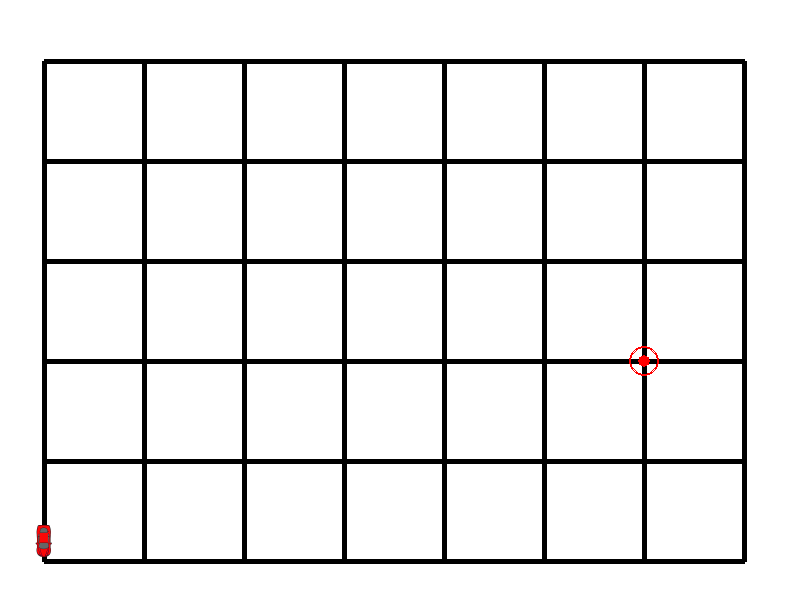
\includegraphics[width=\textwidth]{planner_world}
\centering
\caption{The planner's world. The smartcab is at position $(1, 6)$, facing South, and a forward move would therefore take it to position $(1, 1)$. The destination is at position $(7, 4)$. Due to the toroidal nature of the world, the smartcab's next move should be \textit{right}, taking it to position $(8, 6)$ and 3 moves away from its destination.}
\end{figure}

\subsection{Algorithm and Techniques}
\label{sec:algos}
\textit{Q-learning description}

For the learning planner of this project, I'll be using the $Q$-learning family of algorithms described in the Reinforcement Learning section of Udacity's Machine Learning Engineer nanodegree. A $Q$-learning algorithm allows an agent to learn an optimal policy from sets of states, actions, next states, and rewards, without being explicitly told which actions are optimal in which circumstances. 

The general form of the $Q$-function is:

\begin{equation}
Q(s, a) = R(s) + \gamma \sum_{s'}{T(s,a,s')}\max_{a'}{Q(s',a')}
\end{equation}

That is, the $Q$-value for a given $(state, action)$ pair is the the reward for that state, $R(s)$, plus the discounted (by the discount factor $\gamma$) expected value of $Q$ for the next state the agent lands in, considering the transition function $T(s,a,s') = Pr(s'|s,a)$ (the probability of landing on state $s'$ coming from state $s$ and performing action $a$) and assuming that, whatever $s'$ is, the agent will pick $a'$ so as to maximize $Q$ from there on.

The $Q$-learning update function is given by:

\begin{equation}
\label{eq:q-update}
\hat{Q}_t(s,a) = (1 - \alpha_t) \hat{Q}_{t-1}(s,a) + \alpha_t(r + \gamma \max_{a'}\hat{Q}_{t-1}(s',a'))
\end{equation}

That is, our estimate of the $Q$-value for the $(state, action)$ pair is updated with the learning rate ($\alpha_t$, which varies over time) by the observed reward ($r$) and our previous estimate of the $Q$-value for the observed next state ($s'$), discounted by $\gamma$ and assuming the agent will pick the action $a'$ that maximizes $Q$ from the next state on.

To implement a $Q$-learning algorithm we need to define the following:

\begin{itemize}
    \item \textbf{A discount factor, $\gamma$}. This will define how future rewards are to be valued in comparison to present rewards.
    \item \textbf{A learning rate, $\alpha$}, and its decay rule. This defines how quickly the agent updates the $Q$-value of each $(state, action)$ pair as it explores the state space.
    \item \textbf{Initial $Q$-values} for the $(state, action)$ pairs. A common strategy to promote exploration by the agent is \textit{optimism in the face of uncertainty}, initializing high $Q$-values that will decrease as the agent explores the world. If the agent always picks the action that yields the largest $Q$-value (see below), this guarantees the agent will be compelled to pick previously unperformed actions.
    \item \textbf{A policy}, or a way for the agent to pick actions based on the updated $Q$-function. Most of the times, the agent should pick the action that yields the largest $Q$-values, thus \textit{exploiting} the knowledge of the state space previously acquired. However, it is also important for the agent to \textit{explore} the state space in order to acquire this knowledge. A compromise may be found by defining a \textbf{decaying exploration rate, $\epsilon$}, and setting the agent to perform a previously unperformed action (typically chosen at random) with probability $\epsilon_t$.
\end{itemize}

The implementation of the $Q$-learning algorithm in this setting will be presented in the \hyperref[sec:implementation]{Implementation section}.

\subsection{Benchmark}
\label{sec:benchmark}
Before implementing the learning planner, I implemented two other planners, whose results will be compared to the learning planner's:

\begin{itemize}
    \item A \textbf{random planner} that selects an action at random at each step.
    \item A \textbf{perfect planner}  that always selects the best possible action, defined as an action that reduces the distance between the agent and the destination. (Depending on the agent's position, more than one action can be the ``best'' under this definition: for instance, if the shortest path to the destination involves going forward and taking a right turn, both actions would be considered as the ``best'' one.)
\end{itemize}

See the implementation of these agents, as well as the learning agent, \hyperref[sec:implementation]{in the Implementation section}.

The tables below summarize these two planners' performance in a simulation with 2000 trials.

\renewcommand{\arraystretch}{1.25}

\begin{center}
   \begin{tabular}{rll}
        \multicolumn{3}{c}{\textbf{Random Planner Results}} \\
        \textbf{Metric}    & \textbf{Sum of rewards}    &\textbf{Steps taken}\\
        Mean               & -99.2                      & 47.9\\
        Standard deviation & 160.9                      & 35.1\\
        Minimum            & -460.0                     & 1.0\\
        Q1                 & -216.0                     & 17.0\\
        Median             & - 59.5                     & 39.5\\
        Q3                 & 40.0                       & 84.0\\
        Maximum            & 100.0                      & 100.0\\
        \multicolumn{3}{r}{Destinations reached: 1752/2000}\\
        \multicolumn{3}{r}{Trials with positive sum of rewards: 741/2000}\\
        \multicolumn{3}{r}{States visited: 744}\\
    \end{tabular}
\end{center}

The random planner reached its destination in approximately 87.5\% of the trials - a good result achieved due to the generous deadline defined: in over 75\% of the time, the random planner needs more than 17 steps to reach the destination, which is more than double the worst case for the perfect planner (see below). Only 37\% of the trials end with a positive sum of rewards for the random planner.  

\begin{center}
   \begin{tabular}{rll}
        \multicolumn{3}{c}{\textbf{Perfect Planner Results}} \\
        \textbf{Metric}     & \textbf{Sum of rewards}   & \textbf{Steps taken}\\
        Mean                & 91.2                      & 3.7\\
        Standard deviation  & 6.0                       & 1.4\\
        Minimum             & 73.0                      & 1.0\\
        Q1                  & 86.0                      & 3.0\\
        Median              & 91.0                      & 4.0\\
        Q3                  & 95.0                      & 5.0\\
        Maximum             & 100.0                     & 7.0\\
        \multicolumn{3}{r}{Destinations reached: 2000/2000}\\
        \multicolumn{3}{r}{Trials with positive sum of rewards: 2000/2000}\\
        \multicolumn{3}{r}{States visited: 244}\\
    \end{tabular}
\end{center}

By contrast, the perfect planner always reaches its destination and always nets a positive sum of rewards. It takes at most 7 steps to reach its destination, which makes sense considering the dimensions of the state and its toroidal nature.\footnote{Since the agent can ``go around the world'', it will need at most $(m+n)/2$ steps to reach any destination.}

One interesting difference between these planners is the number of states visited, much larger for the random planner. This makes sense because, with a perfect planner, there is no exploitation: the correct action will always be taken, so any state involving a wrong action (i.e., an action that leads to an increase of the distance between the agent and its destination) is automatically discarded. This amounts to a significant reduction of the state space the agent will experience, but it does not detract in any way from the agent's performance. 

\section{Methodology}

\subsection{Data Preprocessing}
There is no data processing in this project, since the input space is created ``from scratch'', based on the code for project 4.

The only step that may be considered as data processing is the function \texttt{get\_distance()}, which returns the absolute sum of a a tuple of North-South and East-West distances. This is necessary to calculate the planner's reward at states in which the agent has not reached its destination, which is defined as the negative of the Manhattan distance between the agent and the destination (see below).

\subsection{Implementation}
\label{sec:implementation}
\textit{Q-learning model (maybe code?) - reward, number of trials, deadline per trial}

\subsubsection{Basic Planner}
\label{subsec:basic}

The basic planner is defined in the \texttt{Planner} class, with the following attributes and methods:

\begin{itemize}
    \item \texttt{initial\_val}: the initial $Q$-value for a previously unknown $(state, action)$ pair. The default value for this attribute is 0.
    \item \texttt{disc\_rate}: the rate used to discount future rewards. The default value is 0.5.
    \item \texttt{learn\_rate\_func}: a function that takes the number of steps already taken by the agent as an argument and returns the learning rate to be used in the next update of the $Q$-table. Its default is $1.0 / (x + 1)$, where \texttt{x} is the number of steps taken by the agent.
    \item \texttt{q\_vals}: the $Q$-table, initialized as an empty dictionary.
    \item \texttt{possible\_actions}: a list of the possible actions the agent can perform: \texttt{forward}, \texttt{left}, or \texttt{right}.
    \item \texttt{update\_qval()}: a method that updates the agent's $Q$-table, in the following way:
    
    \begin{itemize}
        \item The number of steps \texttt{t} (passed to the method as an argument) is passed to \texttt{learn\_rate\_func()} (see above), which returns the learning rate to be used
        \item The current $Q$-value of the $(state, action)$ pair in the experience tuple (passed to the function as an argument) is retrieved
        \item The next state in the experience tuple is passed to the planner's \texttt{policy()} method (see below), which returns the next action to be performed.
        \item The updated $Q$-value for the $(state, action)$ pair is calculated using the $Q$-update function presented in \hyperref[eq:q-update]{equation \ref{eq:q-update}}.
        \item[] This function could have been implemented only for the learning planner; however, implementing it in the basic planner guarantees that we can check how many states every planner visited.
    \end{itemize}
\end{itemize}

\subsubsection{Operating Planners}

The basic planner described above lacks a \texttt{policy()} method - that is, a method to define the action to be performed given a state. I describe below the policy that defines each type of planner: the perfect and random planners whose results were presented in the \hyperref[sec:benchmark]{Benchmark section}, and the learning planner whose results will be presented in the \hyperref[sec:results]{Results section}.

\begin{itemize}
    \item \textbf{Random planner}: The policy for this planner consists of randomly picking one of the three possible actions.
    \item \textbf{Perfect planner}: The policy consists of always picking an action that reduces the Manhattan distance between the agent and its destination.
    \item \textbf{Learning planner}: The policy consists of picking one of the best actions according to the $Q$-table. Given a state $s$, the learning planner checks the $Q$-value of all $(state, action)$ pairs for which the state is $s$, and picks the action that maximizes this value, breaking ties randomly.
\end{itemize}


\subsection{Refinement}

The refinement of the model involved adjusting the parameters of the $Q$-update function. After a learner with the default parameters  \hyperref[subsec:basic]{presented above} was tested, the learning function rate was modified to return $1.0 / ln(x + 1)$. The results of both models are presented in the \hyperref[sec:results]{Results section}.

\section{Results}
\label{sec:results}

The tables below summarize the two learners' performance in a simulation with 2000 trials.

\renewcommand{\arraystretch}{1.25}

\begin{center}
   \begin{tabular}{rll}
        \multicolumn{3}{c}{\textbf{Original Learner Results}} \\
        \textbf{Metric}    & \textbf{Sum of rewards}    &\textbf{Steps taken}\\
        Mean               & 80.3                       & 5.7\\
        Standard deviation & 23.3                       & 4.4\\
        Minimum            & -195.0                     & 1.0\\
        Q1                 & 73.0                       & 3.0\\
        Median             & 86.0                       & 5.0\\
        Q3                 & 95.0                       & 7.0\\
        Maximum            & 100.0                      & 59.0\\
        \multicolumn{3}{r}{Destinations reached: 2000/2000}\\
        \multicolumn{3}{r}{Trials with positive sum of rewards: 1974/2000}\\
        \multicolumn{3}{r}{States visited: 727}\\
    \end{tabular}
\end{center}

The original learner had very good results, reaching the destination in all trials and netting a positive sum of rewards over 98\% of the time. However, its results are not as good as the perfect planner's; its median sum of rewards is somewhat smaller, for instance, while the median number of steps taken is a little larger. In other words, this learner converges to a good policy, but not a perfect one.

\begin{center}
   \begin{tabular}{rll}
        \multicolumn{3}{c}{\textbf{Final Learner Results}} \\
        \textbf{Metric}     & \textbf{Sum of rewards}   & \textbf{Steps taken}\\
        Mean                & 89.2                      & 4.1\\
        Standard deviation  & 17.0                      & 3.5\\
        Minimum             & -376.0                    & 1.0\\
        Q1                  & 86.0                      & 3.0\\
        Median              & 91.0                      & 4.0\\
        Q3                  & 95.0                      & 5.0\\
        Maximum             & 100.0                     & 100.0\\
        \multicolumn{3}{r}{Destinations reached: 1999/2000}\\
        \multicolumn{3}{r}{Trials with positive sum of rewards: 1993/2000}\\
        \multicolumn{3}{r}{States visited: 716}\\
    \end{tabular}
\end{center}

The final learner missed its destination in 1 of the 2000 trials simulated, and netted a negative sum of rewards in 7 trials. However, the percentiles of its results are identical to the perfect planner's. This indicates that a simple change in the learning rate decay was sufficient to achieve a perfect planning strategy through reinforcement learning. 

\section{Conclusion}

\subsection{Free-Form Visualization}
Figures 2 and 3 show the rolling means over 100 trials of all the planner's results (sum of rewards and steps taken per trial).

\begin{figure}
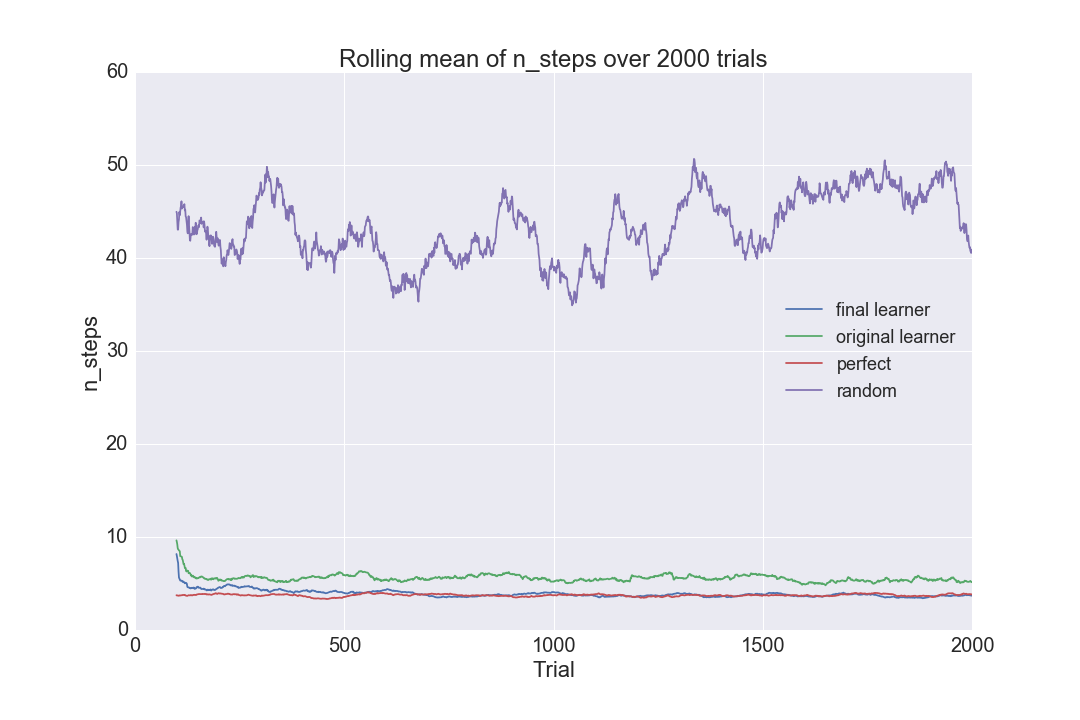
\includegraphics[width=\textwidth]{roll_mean_n_steps}
\centering
\caption{The rolling means over 100 trials of the number of steps taken at each trial by the planner. Taking more than 7 steps necessarily indicates a less than perfect strategy, since, in an $8\times6$ grid world, any position may be reached from any other in 7 steps or less. A number of steps of 100 - the deadline in the simulation - indicates the destination was not reached.}
\end{figure}

\begin{figure}
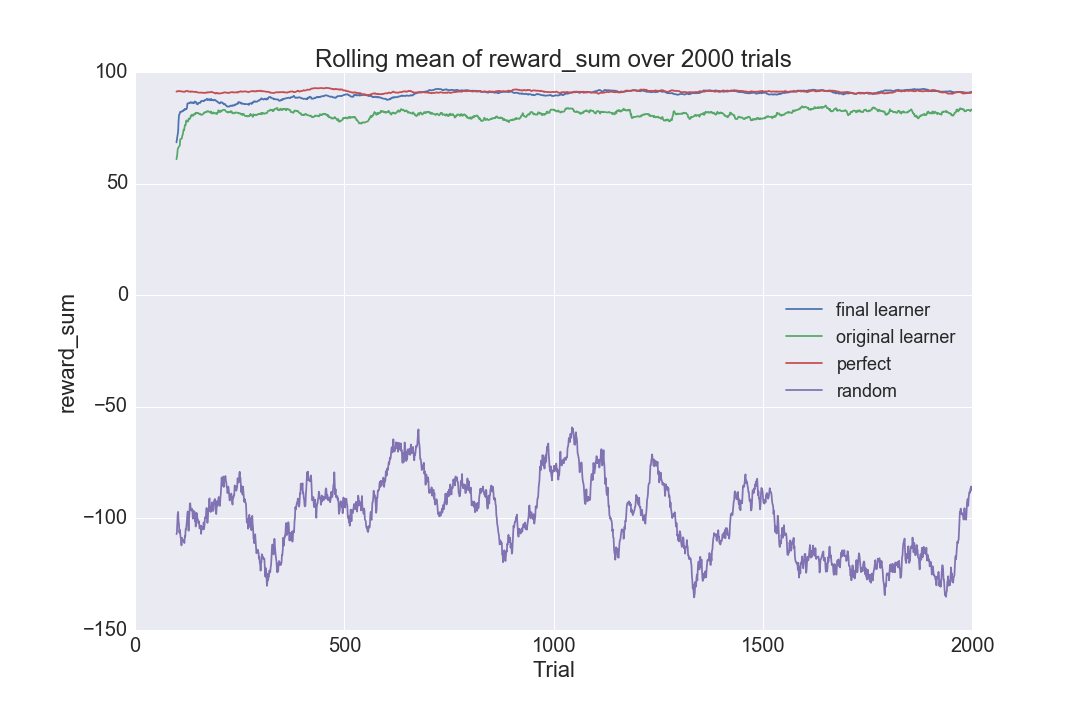
\includegraphics[width=\textwidth]{roll_mean_reward_sum}
\centering
\caption{The rolling means over 100 trials of the sum of rewards for each trial.}
\end{figure}

The figures show how each learner's behavior changes over time:

\begin{itemize}
    \item The \textbf{perfect planner}'s behavior is the same throughout the trials. This is to be expected, since this instance does not learn from experience. Since the perfect planner always performs an action that leads to the decrease of the distance between the agent and its destination, its behavior is ideal in all trials. The small fluctuations that happen are due to different initial positions of the agent and its destination, which modify the distance between these two points and consequently the number of steps taken by the agent in a given trial, as well as the overall sum of rewards it receives.
    \item The \textbf{random planner}'s behavior also does not change over time, again because the planner does not learn from experience. But its results fluctuate wildly over time: the random nature of the planner allows for "lucky" or "unlucky" streaks, during which it may seem as if the agent's behavior is improving or worsening. However, there is no trend in the planner's erratic behavior, which remains fluctuating around a stationary value for both the overall sum of rewards and the number of steps taken at each trial.
    \item The \textbf{original learner}'s results improve markedly at the beginning of the simulation, over the first 200 trials or so, and then become stationary slightly below the perfect planner's results. This is in line with what we saw from the statistics of the original planner's results: the planner converges to a good, but suboptimal, behavior.
    \item The \textbf{final learner}'s results also improve markedly at the beginning of the trial; but they continue to improve, in a smaller rate, until a little after the $500^{th}$ trial they become indistinguishable from the perfect planner's results. This is also in line with my previous analysis of the final learner's statistics: after a while, this learner converges to an optimal policy. 
\end{itemize}

\subsection{Reflection}

When I started this project, the grid world and the planners were all defined as a series of functions. Revisiting the project after a while, it became clear to me that this would lead to code repetition and confusion, so I decided to implement the \texttt{PlannerWorld} and \texttt{Planner} classes described above. This made for a much simpler and clearer code.

It was also after some time away from the project that I decided to modify the learning rate decay, and I was surprised by, and very satisfied with, the results. Since the original learner already had results close to the perfect planner, I believed there was very little room for improvement in the learner, and that any improvement would be difficult to perceive. However, it was clear from the start that the optimized learner had achieved a policy comparable to that of the perfect planner.

My first version of the final planner also included a modification of the $Q$-values assigned to unseen $(state, action)$ pairs. Following the "optimism under uncertainty" method, I increased this initial value to make the learner more exploratory. However, once I modified the learning rate decay I saw this was the only modification necessary, so I returned the initial value to 0 for my final planner.

\subsection{Improvement}

In the Machine Learning Engineer's project 4, I had to teach a smartcab to respect traffic rules and follow the waypoints provided by a planner. In this project, I came up with a learning planner that would be able to pass these waypoints along to an agent.

However, the planner I implemented here does not consider what the environment around the smartcab is. Adding this dimension to the planner may improve its results, since the planner may realize, for instance, that an action is better than another because, while both reduce the agent's distance to its destination, only one of them can be performed immediately. This way the agent may be able to escape traffic and red lights.\footnote{For instance, suppose the destination is Northeast of the agent and that the agent is facing North. In this situation, moving forward and turning right would both decrease the agent's distance to its destination. However, if the light is red at the agent's intersection and there's no more traffic, it can only move right. A planner that was aware of the environment around the agent could, in this situation, prefer to tell the smartcab to turn right, an action that can be immediately performed.}

A more prosaic improvement of the project would be leveraging modular arithmetic to write cleaner versions of the planner world's \texttt{get\_delta()} method and the perfect planner's \texttt{policy} method, both of which seem to me unnecessary long and convoluted.

Finally, there are two ways to modify the project that may be fun:
\begin{itemize}
    \item The smartcab's world may not be toroidal. In this setting, an action that would take the smartcab away from the grid may be ignored - or it may cause an accident, with the immediate failure to reach the deadline (and a heavy penalty!).
    \item Obstacles may be added to the grid world, so that the agent is unable to occupy certain positions. This would turn the grid into a maze, with the planner learning little by little the best ways around the walls.
\end{itemize}
\end{document}